\vbox{%
\begin{lstlisting}[language=Python, caption=Súbor \lstinline|../ICH1R.ipynb cell:02|]
import numpy as np
import matplotlib.pyplot as plt

# Parametre
b_0 = 1
a_0 = 1

# Súradnice bodov na x-ovej osi
plotData_x = np.arange(0, 10, 0.1)

# Výpočet hodnôt na y-ovej osi v zmysle danej časovej funkcie
plotData_y = b_0 * np.exp(-a_0 * plotData_x) \end{lstlisting}
}%end of vbox
\vbox{%
\begin{lstlisting}[language=Python, caption=Súbor \lstinline|../ICH1R.ipynb cell:03|]
# Kreslenie grafu
plt.plot(plotData_x, plotData_y)
plt.xlabel('čas $t$')
plt.ylabel('$y(t)$')
plt.show() \end{lstlisting}
\begin{center}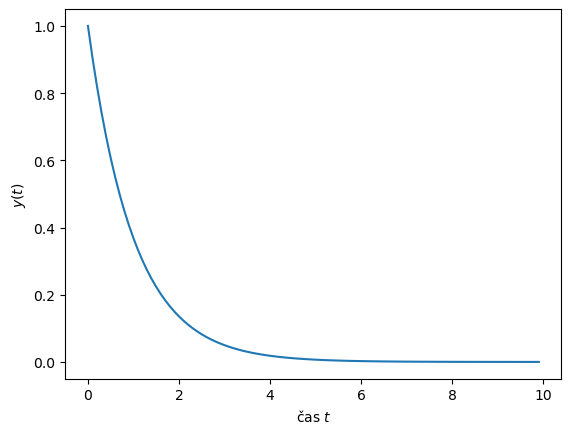
\includegraphics[width=0.68\textwidth]{ICH1Ripynb_cell03out.png}\end{center}}%end of vbox
\vbox{%
\begin{lstlisting}[language=Python, caption=Súbor \lstinline|../ICH1R.ipynb cell:04|]
# Obrázok pre hlavný text
figName = 'ICH_SS1R'
figNameNum = 0
exec(open('./figjobs/figJob_01.py', encoding='utf-8').read()) \end{lstlisting}
}%end of vbox
\vbox{%
\begin{lstlisting}[language=Python, caption=Súbor \lstinline|../ICH1R.ipynb cell:05|]
# Zmeňme hodnotu parametra a_0
a_0 = 0

# Výpočet hodnôt na y-ovej osi v zmysle danej časovej funkcie
plotData_y = b_0 * np.exp(-a_0 * plotData_x) \end{lstlisting}
}%end of vbox
\vbox{%
\begin{lstlisting}[language=Python, caption=Súbor \lstinline|../ICH1R.ipynb cell:06|]
# Kreslenie grafu
plt.plot(plotData_x, plotData_y)
plt.xlabel('čas $t$')
plt.ylabel('$y(t)$')
plt.show() \end{lstlisting}
\begin{center}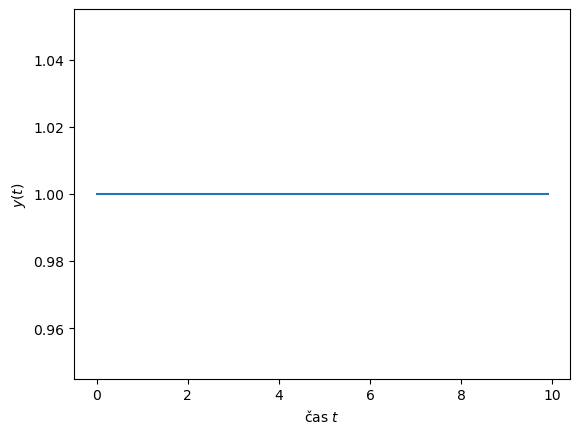
\includegraphics[width=0.68\textwidth]{ICH1Ripynb_cell06out.png}\end{center}}%end of vbox
\vbox{%
\begin{lstlisting}[language=Python, caption=Súbor \lstinline|../ICH1R.ipynb cell:07|]
# Obrázok pre hlavný text
figName = 'ICH_AS1R'
figNameNum = 0
exec(open('./figjobs/figJob_01.py', encoding='utf-8').read()) \end{lstlisting}
}%end of vbox
\vbox{%
\begin{lstlisting}[language=Python, caption=Súbor \lstinline|../ICH1R.ipynb cell:08|]
# Zmeňme hodnotu parametra a_0
a_0 = -1

# Výpočet hodnôt na y-ovej osi v zmysle danej časovej funkcie
plotData_y = b_0 * np.exp(-a_0 * plotData_x) \end{lstlisting}
}%end of vbox
\vbox{%
\begin{lstlisting}[language=Python, caption=Súbor \lstinline|../ICH1R.ipynb cell:09|]
# Kreslenie grafu
plt.plot(plotData_x, plotData_y)
plt.xlabel('čas $t$')
plt.ylabel('$y(t)$')
plt.show() \end{lstlisting}
\begin{center}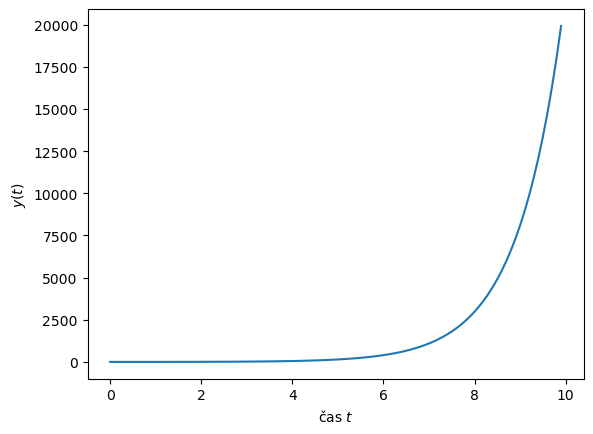
\includegraphics[width=0.68\textwidth]{ICH1Ripynb_cell09out.png}\end{center}}%end of vbox
\vbox{%
\begin{lstlisting}[language=Python, caption=Súbor \lstinline|../ICH1R.ipynb cell:10|]
# Obrázok pre hlavný text
figName = 'ICH_unstable1R'
figNameNum = 0
exec(open('./figjobs/figJob_01.py', encoding='utf-8').read()) \end{lstlisting}
}%end of vbox
